\chapter{Introduction}

The problem of bootstrap percolation was first introduced in the 1970s by Chalupa et al. \cite{chalupa:1979} as a simplified model for the behavior of ferromagnetic fields. In their original paper, the authors describe bootstrap percolation as the stabilization of a probabilistically occupied lattice, where each occupied site must be adjacent to at least $m$ occupied neighbors. A re-rendering of the examples given in the original 1979 paper is presented in figures 1 and 2. 

In this original problem, the authors are interested in the structural patterns of these stable arrangements. Put differently, given a set of randomly distributed occupants on a $d$-dimensional lattice, what configuration can we expect these occupied sites to fall into, subject to the constraint that each occupied site is adjacent to at least $m$ other occupants? In this construction, a probabilistically populated lattice is iteratively de-populated until it reaches a stable state. 

Alternatively, we might consider the behavior of a population as it grows, instead of shrinks. In this model, it is useful to consider the population as harboring an infection that steadily spreads from site to site, subject to population density. We shall consider these infections to take place on a graph, with vertices representing members of our population (sites), and edges indicating adjacency. In formal terms: let $G$ be a graph and $A_0 \subseteq V(G)$ be a set of initially infected vertices. Iteratively, at every time step, infect those vertices of $G$ with at least $r$ infected neighbors. For all $t > 0$, let $A_t$ be the set of infected vertices at time step $t$. We then have
$$A_t = A_{t-1} \cup \{v \in V(G) : |N_G(v) \cap A_{t-1} \geq r\},$$
where $N_G(v)$ is the set of vertices adjacent to $v$ in $G$. We define the \emph{closure} of $A_0$ under $r$-neighbor bootstrap percolation to be $[A_0] = \bigcup_{t=0}^{\infty} A_t$. This is analogous to the stable states introduced in \cite{chalupa:1979}. We say that $A_0$ \emph{percolates} or is \emph{lethal} if $[A_0] = V(G)$. We note that under these rules, it is not possible for vertices to become uninfected. 

Perhaps the most natural extremal question regarding $r$-neighbor bootstrap percolation is that of determining the size of the smallest percolating set $A_0 \subseteq V(G)$, for a given graph $G$. We represent this quantity by $m(G,r)$. There has been a great deal of work done on establishing the value of $m(G,r)$ for various classes of graphs and values of $r$ (see \{citations, citations, etc., etc.\}). These results are incompletely summarized in table \ref{tab:known_bounds}, and a selection of particularly noteworthy proofs are presented in detail in the following section.

\begin{table}[]
\centering
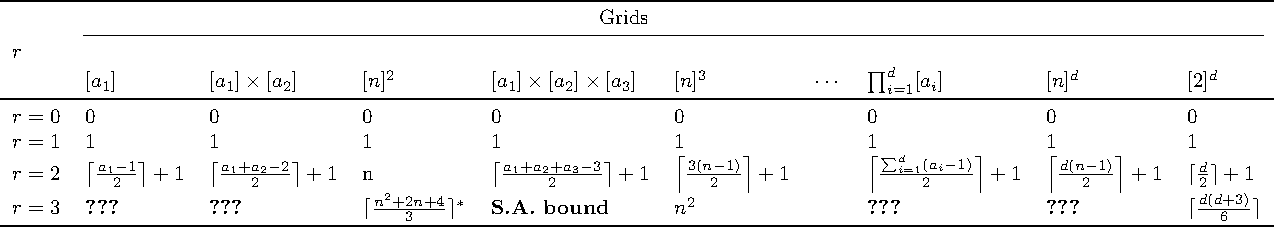
\includegraphics[width=\textwidth,origin=c]{tables/1/known_bounds.pdf}
\caption{A summary of known bootstrap percolation results for grids and the torus, $r \in \{0,1,2,3,d\}$.}
\label{tab:known_bounds}
\end{table} 

We end this introduction with the presentation of a delightful question about the cardinality of $2$-neighbor percolating sets on the two-dimensional lattice. The interested reader in encouraged to find a solution on their own; however, a proof of the result is presented at the beginning of the following section.
\begin{question}
Let $(n,n)$ represent the $n \times n$ lattice, given by $G = P_n \times P_n$. What is $m(n,n,2)$?
\end{question}

\section{Minimum percolating sets and bounds}

\subsection{Foundations}

Let us build some intuition for the behavior of percolating sets on the two-dimensional lattice. Figure \ref{fig:5x5x1} illustrates the percolation time-steps for an arbitrary initial infection on the graph $G=P_5 \times P_5$, where $r=2$. (In general, we shall refer to the $d$-dimensional lattice with sides $a_1, \dots, a_d$ as the $d$-tuple $(a_1, \dots, a_d)$. The standard notation is $\prod_{i=1}^d a_i$.) 

\begin{figure}[]
\centering
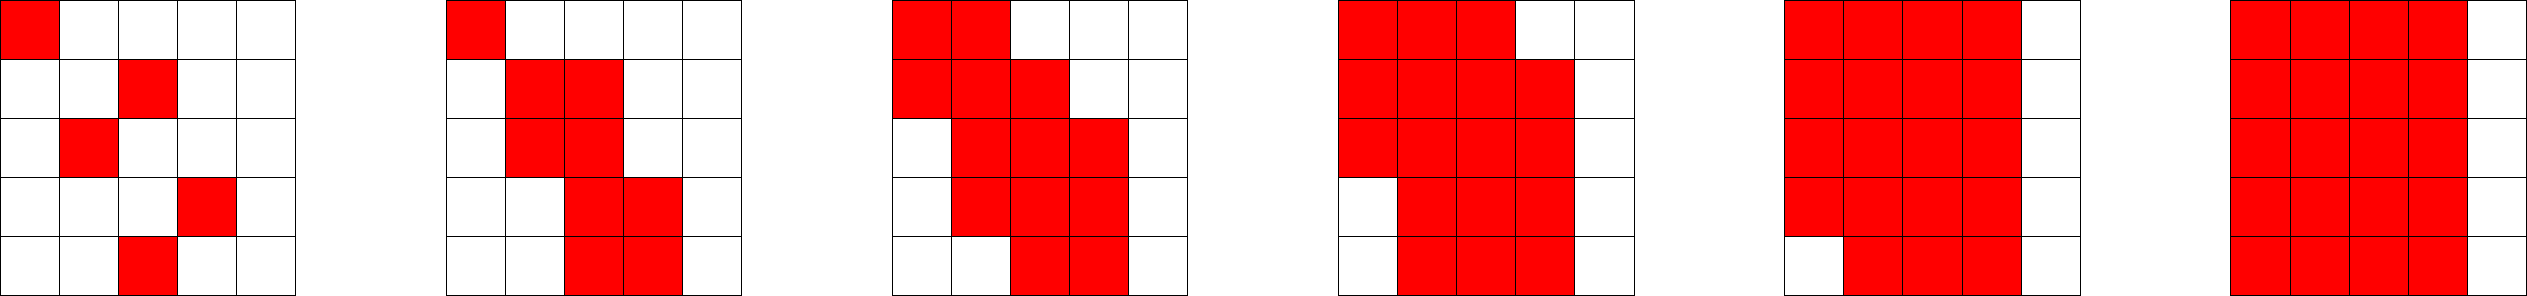
\includegraphics[width=\textwidth]{figures/1/5x5x1.pdf}
\caption{Percolation time-steps for an arbitrary initial infection on the $5 \times 5$ lattice, $r=2$.}
\label{fig:5x5x1}
\end{figure} 

Note that this configuration fails to infect the entire grid; that is, the initial infection is not lethal. Heuristically, this appears to be a consequence of the fact that infected cells are unable to access the healthy cells in the rightmost column. We might, therefore, hypothesize that an initial infection must somehow ``span" the entire lattice. A potential ``spanning" construction is illustrated in figure \ref{fig:5x5x1_improved}. Observe that at each time-step, the infection spreads out laterally from the initial diagonal. It is a simple exercise to verify that this construction is lethal on all $(n,n)$ grids for $r=2$. We also note that a similar construction is lethal on all $(n,m)$ grids for $r=2$ (figure \ref{fig:8x4x1}).

\begin{figure}[]
\centering
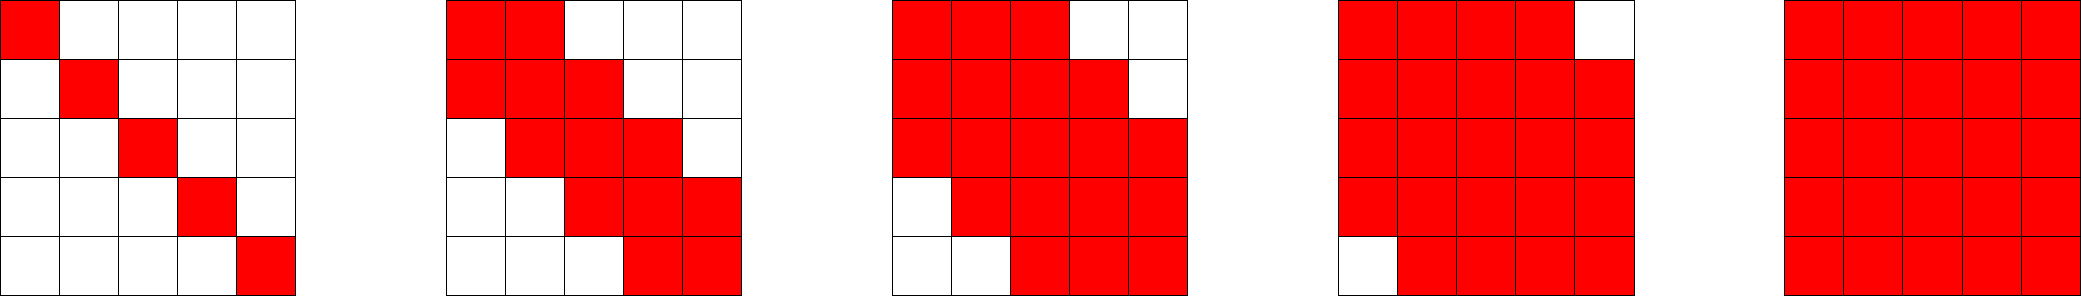
\includegraphics[width=\textwidth]{figures/1/5x5x1_improved.pdf}
\caption{Percolation time-steps for a ``spanning" initial infection on the $5 \times 5$ lattice, $r=2$.}
\label{fig:5x5x1_improved}
\end{figure} 

\begin{figure}[]
\centering
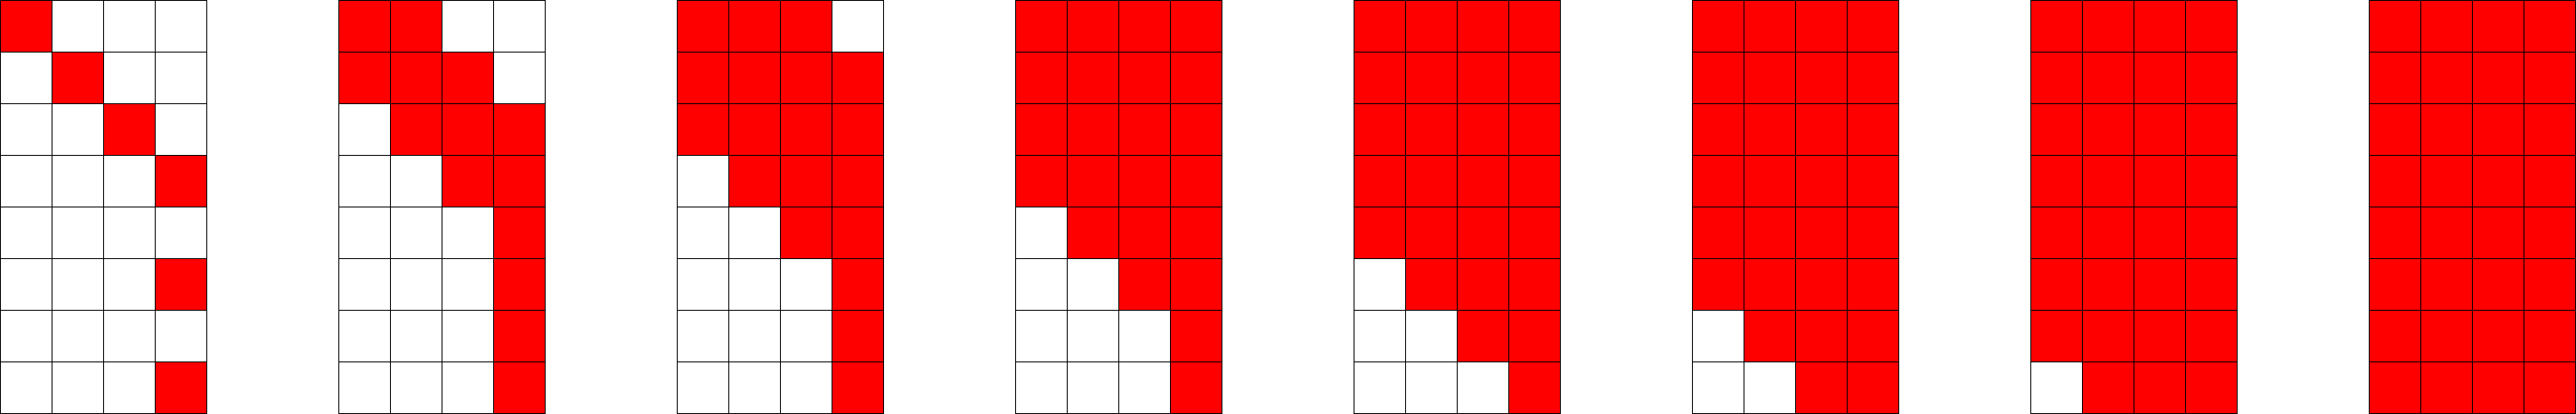
\includegraphics[width=\textwidth]{figures/1/8x4x1.pdf}
\caption{A lethal infection on the $8 \times 4$ lattice, $r=2$.}
\label{fig:8x4x1}
\end{figure} 

The $(n,n)$ construction can be generalized to any dimension. Specifically, we have:

\begin{prop}
\label{prop:nxn_lower_bound}
For all $n,d \geq 1$, 
$$m([n]^d, d) \leq n^{d-1}.$$
\end{prop}
This result has been known since at least Pete \cite{pete:1997}, although the particular constructions are difficult to render in general. The following proof (appearing in \cite{przykucki:2019}, but known in bootstrap percolation ``folklore" for much longer) elegantly shows that this bound is tight.

\begin{thm}
\label{thm:tight_perimeter}
For all $n,d \geq 1$, 
$$m([n]^d, d) = n^{d-1}.$$
\end{thm}

\begin{proof}
The upper bound follows from proposition \ref{prop:nxn_lower_bound}. The lower bound is given by a generalization of the famous ``perimeter argument". Suppose $d=2$ and consider an embedding of $G=[n]^d$ in the $n\times n$ grid. Let $A_0 \subseteq V(G)$ be a set of initially infected cells. We claim that the total perimeter of all infected regions in $G$ is monotonically decreasing as a function of the time-step $t$. Consider an arbitrary healthy cell $c$. In order for $c$ to become infected, at least two of its edges must abut infected cells. However, this implies that (upon infection of $c$) these edges are absorbed within the newly expanded infected region, thereby reducing the perimeter of infection by two. As $c$ contains at most two un-absorbed edges, the perimeter of infection cannot increase. 

Since a lethal set will infect the entire grid, and therefore have a final perimeter of infection of $4n$, it follows that the perimeter of infection of $A_0$ must be at least $4n$, and so $m([n]^2, 2) \geq n.$

The same argument generalizes nicely to higher dimensions. Simply observe that for a given hypercube cell to become infected, it must donate at least $d$ of its $2d$ hyperplane faces to the infected region, thereby at most maintaining the current $(d-1)$-perimeter of infection.
\end{proof}

We note that the perimeter argument extends directly to rectangular grids; however, the problem of obtaining tight constructions, should they exist, is largely unsolved and will be the main focus of this thesis. The following proposition, which we refer to informally as the \emph{surface area bound} or \emph{S.A. bound}, provides a lower bound on the size of lethal sets for $d$-dimensional rectangular grids where $r=d$.

\begin{prop}
\label{prop:SA_bound}
For $d \geq 1$ and $a_1, \dots, a_d \geq 1$,
$$m(a_1, \dots, a_d, d) \leq \frac{\sum_{i=1}^d \prod_{j \neq i} a_j}{d}.$$
\end{prop}

\begin{proof}
Observe that the expression
$$\frac{\sum_{i=1}^d \prod_{j \neq i} a_j}{d}$$
is precisely the high-dimensional perimeter of the grid graph $(a_1, \dots, a_d)$. The bound follows from the perimeter argument in theorem \ref{thm:tight_perimeter}. 
\end{proof}

In \{some chapter of this thesis\}, we will prove that this bound is tight in the case where $d=3$ and $d_1,d_2,d_3 \geq 8$. We fully expect that this bound can be incrementally diminished; however, we feel that such small improvements do not at this time justify the effort required to obtain additional constructions. 

In the remainder of this section, we shall present a number of additional bootstrap percolation results for different classes of grid graphs.

\subsection{Additional results}

Recall from the previous section that $m(n,n,2) = n$, where the tight construction for the lower bound is given by a diagonal infection expanding laterally outwards. In a paper by Balogh and Bollobas \cite{balogh:2006}, this result is generalized to all $d$-dimensional hypercubes $(a_1, \dots, a_d)$, $a_i \geq 1$. 

\begin{thm}
For $d \geq 1$ and $a_1, \dots, a_d \geq 1$, 
$$m(a_1, \dots, a_d, 2) = \ceil*{\frac{\sum_{i=1}^d (a_i-1)}{2}}+1.$$
\end{thm}

\begin{proof}
\end{proof}

As suggested by table \ref{tab:known_bounds}, general results become quite sparse for $r \notin \{2,d\}$. A nice result from Morrison and Noel resolves the question of $r=3$ for hypercubes $P_2^d$ of dimension $d \geq 3$. 

\begin{thm}
For $d \geq 3$ and $a_1 = \dots = a_d = 2$, 
$$m(a_1, \dots, a_d, 3) = \ceil*{\frac{d(d+3)}{6}}.$$
\end{thm}

\begin{proof}
\end{proof}

However, the issue of determining $m(a_1, \dots, a_d, r)$ is largely unresolved. Furthermore, good lower bounds for $r \neq d$ are conspicuously absent. 

